\section{Physischer Entwurf}
Der Vorgang ist iterativ. Tuning erfolgt während des laufenden Betriebs.

\begin{itemize}\itemsep0em
	\item Speichermedium wählen (RAID 0, 1, 5)
	\item Zugriffsart
	\item Block-, Seitenzuweisung, Verteilung der Daten
	\item Indexierung
	\item Monitoring
	\item Denormalisierung
\end{itemize}

\subsection{Speicherhierarchie}
Je schneller, desto kleiner, desto teurer ...
\begin{enumerate}\itemsep0em
	\item Cache Speicher
	\item Arbeits-, Programmspeicher
	\item Massenspeicher, Festplatte, USB-Stick
	\item Archiv-Speicher (Magnetbänder, optische Platten)
\end{enumerate}

\subsubsection{Festplatten}
%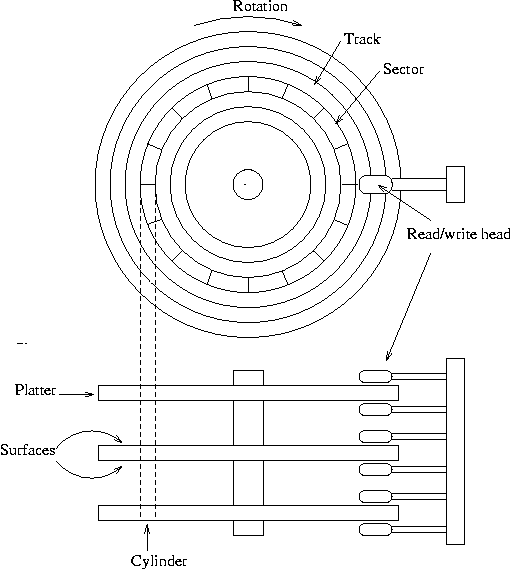
\includegraphics[width=\linewidth]{hd-schematic.png}
bestehen aus einem Plattenstapel. Eine Platte ist in Spuren (Tracks), diese in Sektoren unterteilt. 
Übereinanderliegende Spuren heissen Zylinder. Mehrere Spuren bilden einen Block.

Daten werden blockweise geschrieben/gelesen. Es werden immer ganze Blöcke übertragen.

Das DBMS stellt einen Disk Space Manager (verwaltet Zugriff auf Sekundärspeicher) und einen Buffer Manager
(verwaltet den Hauptspeicher) zur Verfügung. Das Betriebssystem gewährt mit dem Platten-Controller den Zugriff.

\subsection{Datenorganisation}
\settowidth{\MyLenA}{Unsortierte Daten~~}
\begin{tabular}{
	@{}p{\the\MyLenA}%
	@{}p{\linewidth-\the\MyLenA}}
	Unsortierte Daten & Sequentielle Suche ($\frac{n}{2}$ Zugriffe)\\
	Sortierte Daten & Binäre Suche ($\log_2 n$ Zugriffe)\\
\end{tabular}\\
$n =$ Anzahl Datensätze. Sortierung nur für ein Kriterium möglich. Indexe sind verschiedene sortierte Verzeichnisse.
Aber: Indexe brauchen zusätzlichen Speicherplatz und müssen gepflegt werden (Update-Query-Tradeoff)
Indexe sind das primäre Optimierungsmittel!

\begin{itemize}\itemsep0em
	\item [$+$] Primärschlüssel (i.\,d.\,R. automatisch)
	\item [$+$] Fremdschlüssel (beschleunigt Joins)
	\item [$+$] Attribute mit häufigen Abfragen und kleinen Resultatmengen
	\item [$+$] Attribute, die oft sortiert ausgegeben werden
	\item [$-$] Attribute, deren Wert sich häufig ändert
	\item [$-$] Grosse Attribute, komplexe Attributkombinationen
\end{itemize}

\subsubsection{Datenorganisationsformen}
\begin{description}
	\item [Heap-Datei] Bei einer Heap-Datei werden die Datensätze unsortiert hintereinander (sequentiell) geschrieben.
	Einfach, aber nur sequentielle Suche ist möglich (Suchen, bis gefunden).
	\item [Hash-Verfahren] Dabei werden die Datensätze unterschiedlichen Bereichen zugeordnet. Innerhalb der Bereiche 
	sind die Datensätze wieder ungeordnet. Die Zuordnung der Datensätze zu den Bereichen erfolgt über eine Hashfunktion.
	Einfach, aber einzelne Bereiche müssen sequentiell durchsucht werden.
	\item [ISAM-Verfahren] Beim ISAM-Verfahren (Index Sequential Access Method) wird neben der eigentlichen Datendatei, 
	die die Datensätze in sortierter Reihenfolge enthält, eine weitere Datei, die so genannte Index-Datei gepflegt. 
	Diese Index-Datei ermöglicht einen beschleunigten Zugriff auf die Daten. Suchen ist sehr schnell, aber die Index-Datei
	muss ständig mit angepasst werden.
	\item [B$^*$-Baum-Verfahren] Betrachtet man die Indexdateien des ISAM-Verfahrens wiederum als Datensätze, so kann zu diesen Datensätzen wiederum eine Indexdatei
	generiert werden. Durch diese Verschachtelung von Indexdateien kommt man zu einer baumartigen Struktur. 
	Merkmale eines B*-Baumes:
	\begin{itemize}\itemsep0em
		\item Jeder Knoten des Baumes kann mehrere Kindknoten haben (Mehrwegbaum)
		\item Der Baum ist ausgeglichen (balancierter Baum)
		\item Die Knoten enthalten nur Verweise und nicht die eigentlichen Daten
	\end{itemize}
	Es gibt so zwar keine grossen Index-Dateien, doch einfügen und löschen ist kompliziert. Die optimale Variante
	für überwiegend lesenden Zugriff.
	\item [Sekundärindex] Index über ein zusätzliches Merkmal. Lesender Zugriff auf zusätzliches Merkmal ist sehr schnell, aber einfügen und
löschen ist noch komplizierter als beim B$^*$-Baum-Verfahren.
\end{description}

\subsection{Anfrageoptimierung}
Die Anzahl Diskzugriffe sind zu minimieren. Dabei werden Abfragebäume visualisiert und mit Hilfe der relationalen Algebra
optimiert (Kommutativität, Relationen mit höherer Kardinalität in die innere Schleife (Nested-Loop-Join), sortieren vor
dem mischen (Sort-Merge-Join), mit Selektion und Projektion Zwischenergebnisse verkleinern.

Die Optimierung hängt oft vom konkreten Datenvolumen ab.

\subsubsection{Regeln}
\begin{itemize}
	\item Verbund ($\Join$), Vereinigung ($\cup$), Durchschnitt ($\cap$) und Produkt ($\times$) 
	sind kommutativ und assoziativ. 
	\item Selektionen sind vertauschbar: $\sigma_P(\sigma_Q(R)) = \sigma_Q(\sigma_P(R))$
	\item Konjunktionen in einer Selektionsbedingung kann in mehrere Selektionen aufgebrochen werden:
	$\sigma_{P_1}(R) \wedge \sigma_{P_2}(R) \wedge \dots \wedge \sigma_{P_n}(R) = \sigma_{P_1}(\sigma_{P_2}(\dots(\sigma_{P_n}(R))))$
	\item Projektion mit Vereinigung vertauschbar: $\pi_L(A \cup B) = \pi_L(A) \cup \pi_L(B)$
	\item Disjunktion in Konjunktion umwandelbar: $\neg (A \wedge B) = \neg A \vee \neg B, \neg (A \vee B) = \neg A \wedge \neg B$
\end{itemize}
Das DBMS nutzt diese Regeln.
\begin{itemize}\itemsep0em
	\item Wenn möglich vor dem Join sortieren
	\item Wenn Nested-Loop-Join notwendig, vor dem Join einschränken ($\sigma, \pi$)
	\item Indexe reduzieren den Aufwand, kosten aber Aufwand ($n \log_n)$).
\end{itemize}

\subsubsection{Optimierter Abfragebaum}
	\begin{tikzpicture}[
		leaf/.style={rectangle, draw=black, fill=black!10, text width=3cm, drop shadow, text centered},
		node/.style={text width=1cm, text centered},
		line/.style={thick, shorten >=2pt},
		node distance=0.5cm
		]
	\node [node] (projection) {\Large{$\pi$} \normalsize Titel};
 	\node [anchor=west, text width=1cm, left=0.5cm of projection] (note0) {Mng: 1};
 	\node [node, below=of projection] (select) {\Large{$\sigma$}};
	\node [anchor=west, text width=1cm, left=0.5cm of select] (note1a) {Mng: 2};
 	\node [anchor=west,text width=2cm, right=0.5cm of select] (note1b) {\small Ta.Aa = Tb.Ab};
 	\draw [line] (projection) -- (select);

 	\node [node, below=of select] (join) {\Large{$\Join$}};
 	\node [anchor=west, text width=2cm, left=0.5cm of join] (note2) {Mng: 3};
 	\draw [line] (select) -- (join);
	\node [below left=0.25cm of join, text width=4cm, text centered] (sigmaBook) {\Large{$\sigma$} \small Fachgebiet\\= \enquote{Theor. Inf.}\\\normalsize{Menge: 3}};
	\node [below right=0.25cm of join, text width=4cm, text centered] (sigmaLector) {\Large{$\sigma$} \small PersNr\\= \enquote{866778}\\\normalsize{Menge: 1}};
 	\node [leaf, below=of sigmaBook] (book) {Buch};
 	\node [anchor=west, text width=2cm, text centered, below=0.5cm of book] (note3) {Mng: 19};
 	\node [leaf, below=of sigmaLector] (lector) {Lektor};
 	\node [anchor=west, text width=2cm, text centered, below=0.5cm of lector] (note4) {Mng: 6};
 	\draw [line] (join) -- (sigmaBook);
 	\draw [line] (join) -- (sigmaLector);
	\draw [line] (book) -- (sigmaBook);
	\draw [line] (lector) -- (sigmaLector);
	\end{tikzpicture}\\
%

\textbf{Anfragebeispiel:}	$\pi_{t1.f1, t2.f1} (\sigma_{t1.f1 = \mbox{\enquote{kriterium}}}(t1 \Join t2))$

